\chapter{Modeling the Effects of Feedback}
TODO

\subsection{Model Extension}
The third and final Aim of the proposal is addressed by developing a model of the human pilot which includes the effects of concurrent bandwidth feedback.
The proposed Model will extend Professor Hess' structural model of the human pilot to include the effects of concurrent bandwidth feedback.
The Structural Model has been extremely successful in predicting human performance through a variety of system dynamics and can predict how performance changes during a pilot's adaptation to changing dynamics.
Hess has developed adaptive logic for the human pilot in a pursuit task which triggers when the pilot notices that vehicle dynamics have changed~\citep{hess_modeling_2009}.
This logic is based off several criteria, which ``must be predicated upon information available to the human [and] the postadapated pilot models must follow the dictates of the crossover model of the human pilot~\citep{hess_modeling_2009}.''
The primary result of the adaptive logic is to increase the resulting crossover frequency of the pilot, effectively making them more responsive, which could be interpreted as more focused on the task.
Our initial approach to adding concurrent bandwidth feedback into the Structural Model will be based off of Hess' approach to modeling human adaptation in pursuit tasks, which is currently ad-hoc in nature, see Figure~\ref{figure:hesspursuit}.

\begin{figure}[tb]
    \begin{center}
        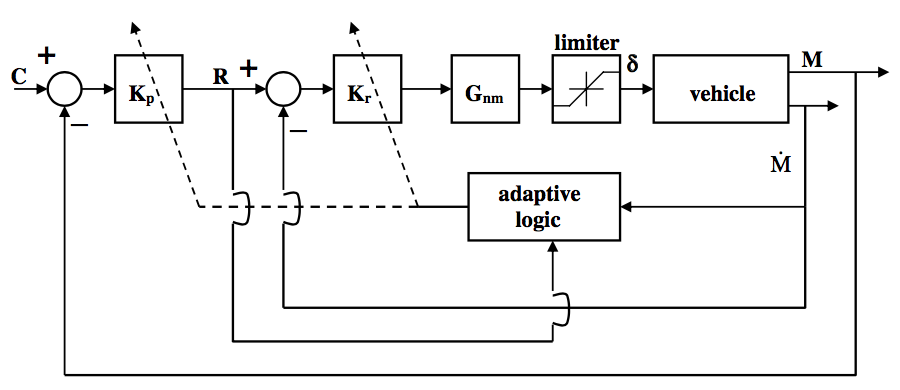
\includegraphics[width=0.8\linewidth]{figures/Screen_Shot_2018-08-09_at_4_15_24_PM.png}
        \caption{Hess' model of the adaptive human pilot, from~\citep{hess_modeling_2009}.}
        \label{figure:hesspursuit}
    \end{center}
\end{figure}

While this model of the adaptive pilot has been successful in predicting changes in performance for a well trained subject, it does not consider how a pilot would behave when they are still in the early stages of training.
Our modified model will include two major changes to Hess' current model:
\begin{itemize}
    \item The adaptation logic will be changed to focus on concurrent bandwidth feedback
    \item The timescale of the adaptation will be significantly longer
\end{itemize}

We propose to modify the adaptive logic to trigger when the pilot is receiving concurrent bandwidth feedback, rather than when a change in system dynamics occurs.
This will require the addition of a feedback loop onto the Structural Model which triggers when the bandwidth feedback is activated.
This loop will likely be based around the $K_e$ gain, which is currently the primary way of setting the crossover frequency in the Structural Model.
This implies that the subjects in our experiments do their primary learning when they are receiving qualitative feedback that their current level of aggressiveness is not sufficient to complete the task.
While there must be a separate loop that adjusts the crossover frequency as learning progresses over the course of several hours, the change in performance we see when subjects use the concurrent bandwidth feedback happens relatively rapidly, within a few minutes.
This is reflected in the delta of performance between subjects in the different groups of our SAFER experiment, even on the first trial, see Figure~\ref{figure:saferdistance}.
This relates to the second required change, the amount of required adaptation time.
Professor Hess' model requires that pilots adapt within a very short time period, on the order of 5 seconds~\citep{weir_model_1966}.
The results of our experiment with SAFER and the three-axis tracking task also suggest relatively short adaptation times, though they are on the order of a few minutes, again see Figure~\ref{figure:saferdistance}.

While it should be noted that this work is in preliminary stages and not scheduled to begin until the Fall Quarter, some early work has been started in preparation for the qualifying examination.
An effort has been made to begin to replicate some of Hess' results.
Working with Professor Hess, we have been able to replicate some of the existing adaptation logic for a two-axis tracking task, and begun exploratory research into modifying the model.
